\documentclass{beamer}
\usepackage[utf8]{inputenc}
\usepackage{graphicx}

%\usetheme{Copenhagen}
\usetheme{Antibes}
\hypersetup{pdfstartview={Fit}}

% Defining a new environment for continual enumerating throught frames
\makeatletter
\newenvironment{cenumerate}{
  \enumerate
  \setcounter{\@enumctr}{\csname saved@\@enumctr\endcsname}
}{
  \expandafter\xdef\csname saved@\@enumctr\endcsname{\the\value{\@enumctr}}
  \endenumerate
}
\newenvironment{cenumerate*}{
  \enumerate
}{
  \expandafter\xdef\csname saved@\@enumctr\endcsname{\the\value{\@enumctr}}
  \endenumerate
}
\makeatother

\title{Joint 3D object recognition and tracking}
\author[Orizio, Rizzini, Zucchelli]{Orizio Riccardo,\\Rizzini Mattia,\\Zucchelli Maurizio}
\date{25 july 2013}
\institute[UniBS]{University of Brescia}
\logo{
\includegraphics[width=15mm]{images/logo.png}}

\begin{document}
  \begin{frame}
    \maketitle
  \end{frame}

  \section{Introduction}
  
  \begin{frame}
    \frametitle{\insertsection}
    The project goal is to realize a joint system of recognition and tracking
    of some features of a previously chosen object which is identified in a
    video.  These features are called \textsc{Label}s.\\
    The sofware is aimed for execution on low performance devices such as the
    iPad, therefore the tracking is necessary due to the high computational
    cost of a pure recognition.\\
  \end{frame}

  \AtBeginSection[]
  {
    \begin{frame}
      \frametitle{Outline}
      \tableofcontents[currentsection]
    \end{frame}
  }

  \section{Manager and overall functioning}

  \begin{frame}
    \frametitle{\insertsection}
	\begin{figure}
		\centering
		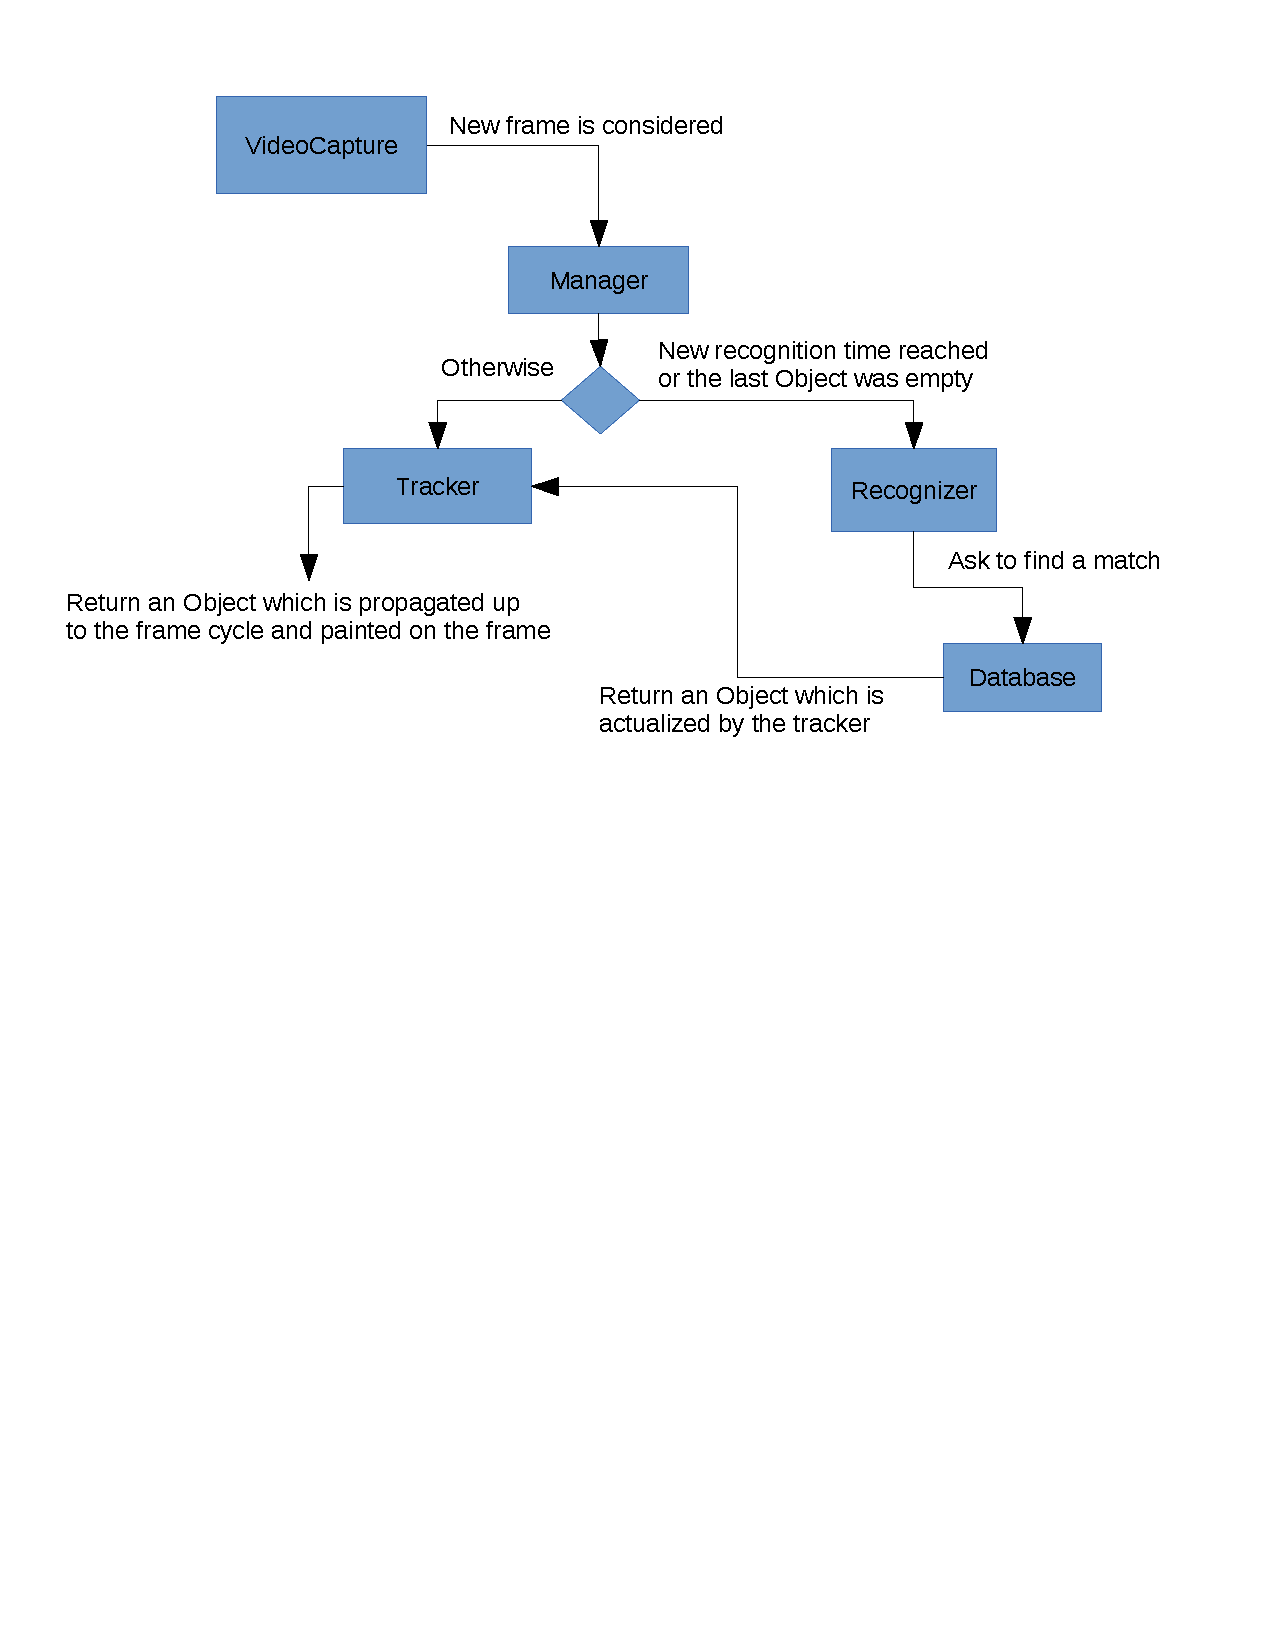
\includegraphics[width=0.8\textwidth]{images/main_flow.pdf}\\
		Fig 1: Graphical presentation of the overall functioning
	\end{figure}
  \end{frame}

  \begin{frame}
    \frametitle{\insertsection}
    The software is designed for concurrent execution.\\
    An object of class \textsc{Manager} handles two objects of class \textsc{Recognizer} and
    \textsc{Tracker}. The first object runs a \emph{thread}.\\
    Every $N$ frames elaborated, the \textsc{Manager} asks the
    \textsc{Recognizer} to perform a full recognition. In the meantime the
    \textsc{Tracker} keeps tracking the \textsc{Label}s starting from the last
    \textsc{Object} given by the \textsc{Recognizer}.\\
  \end{frame}

  \begin{frame}
    \frametitle{\insertsection}
    When the \textsc{Recognizer} has finished it returns an \textsc{Object}
    which contains the positions of the \textsc{Label}s in the moment in which
    the recognition started. These positions are then \emph{actualized} by the
    \textsc{Tracker} and the \textsc{Object} is updated with the actualized positions.\\
	The \textsc{Object} is then used as a reference to paint the \textsc{Label}s on the
	frame and show the result to video.
  \end{frame}

  \section{Recognition}

  \begin{frame}
    \frametitle{\insertsection}
    To perform recognition, \emph{SIFT} descriptors are used since, in our
    tests, they seemed to perform better than the \emph{SURF} ones without any
    computational disadvantage.\\
  \end{frame}

  \subsection{Database}
  
  \begin{frame}
    \frametitle{\insertsection\ - \insertsubsection}
    The recognition bases itself on a \textsc{Database}.\\
    This \textsc{Database} supports serialization of the structures used for
    recognition. At the program start, a \textsc{Database} name is provided:
    if this name corresponds to a serialized \textsc{Database}, the
    \textsc{Database} is loaded; otherwise it is trained.\\
  \end{frame}

  \begin{frame}
    \frametitle{\insertsection\ - \insertsubsection}
    The \textsc{Database} training is performed through the analysis of a group
    of sample images depicting the object from various points of view.\\
    To every image is also associated a text file which contains the absolute
    positions of the various \textsc{Label}s in the referenced sample.\\
    Every sample image is loaded, from every image \emph{SIFT} features are
    extracted, descriptors computed and label positions loaded. Everything
    is then saved in three structures and serialized.\\
    At the end of the training or load phase, a \emph{FLANN} based matcher is
    trained based on all the samples descriptors.\\
  \end{frame}

  \subsection{Matching}

  \begin{frame}
    \frametitle{\insertsection\ - \insertsubsection}
    To perform a match on a frame, the following steps are executed:
    \begin{cenumerate*}
      \item The SIFT features and descriptors are extracted from the frame.
      \item The descriptors are matched using the \emph{FLANN} matcher with
        a \emph{knnMatch} method.
      \item The matches are searched to identify the sample which has got 
        the maximum number of matches. The only informations considered in
        the database are now those regarding this sample.
      \item The matches of that sample are extracted and filtered using the
        \emph{NNDR} criteria.
    \end{cenumerate*}
  \end{frame}

  \begin{frame}
    \frametitle{\insertsection\ - \insertsubsection}
    \begin{cenumerate}
      \item If the remaining matches are less than a threshold, then the
	 	match ends with nothing found (empty \textsc{Object} is given back);
      \item Otherwise the keypoints related to the matches in the database and
        the frame are used to estimate an homography with \emph{RANSAC}.
      \item If it is valid (the inliers ratio over the total points used by
        \emph{RANSAC} is at least 50\%), the homography is used to remap the positions
        of the labels in the frame. Those positions are added to an
        \textsc{Object} which is passed back to the \textsc{Manager}.
    \end{cenumerate}
  \end{frame}

  \begin{frame}
    \frametitle{\insertsection\ - \insertsubsection}
	\begin{figure}
		\centering
		
\includegraphics[width=0.8\textwidth]{images/sample.jpg}\\
		Fig 2: Example image
	\end{figure}
  \end{frame}

  \begin{frame}
    \frametitle{\insertsection\ - \insertsubsection}
	\begin{figure}
		\centering
		
\includegraphics[width=0.8\textwidth]{images/sampleKeypoints.jpg}\\
		Fig 3: Detected keypoints
	\end{figure}
  \end{frame}

  \begin{frame}
    \frametitle{\insertsection\ - \insertsubsection}
	\begin{figure}
		\centering
		
\includegraphics[width=0.8\textwidth]{images/sampleLabels.jpg}\\
		Fig 4: Detected Labels
	\end{figure}
  \end{frame}

  \subsection{Match filtering considerations}

  \begin{frame}
	\frametitle{\insertsection\ - \insertsubsection}
	The matching process implements multiple checks to determine if everything
	is going fine.\\
	The NNDR and inliers ratio checks are strictly connected to each other
	as by adopting a less restrictive NNDR check, more bad matches are allowed
	and therefore RANSAC works on more outliers (decreasing the inliers ratio).
	We've found that a NNDR value of 60\% works fine since when the object is
	standing still in front of the camera, RANSAC works with an inlier ratio
	between 95\% and 100\%.
  \end{frame}

  \begin{frame}
  	\frametitle{\insertsection\ - \insertsubsection}
	On the other hand, we found that the right threshold of remaining matches
	after the NNDR filtering is strictly connected to the quality of the video
	source used as input.\\
	In particular we found that a higher quality source is likely to produce
	more matches that pass the NNDR test, so the threshold should be raised
	up a bit (generally somewhere between 14 and 20).
  \end{frame}

  \section{Tracking}

  \begin{frame}
    \frametitle{\insertsection}
    The tracking of the \textsc{Object} consists of two principal parts:
    \begin{enumerate}
      \item The effective tracking of the \textsc{Object} between two
        successive frames.
      \item The \emph{actualization} of the \textsc{Object} received by the
        \textsc{Recognizer}.
    \end{enumerate}
  \end{frame}

  \begin{frame}
    \frametitle{\insertsection}
    To track an object, \emph{GFTT} (Good Features To Track) are used:
    these features are extremely fast to calculate and provide optimal results
    in tracking application.\\
    The algorithm works on the whole frame: the features are associated to the
    new frame using Lucas-Kanade's method for \emph{optical flow} estimation,
    then, for every \textsc{Label}, the nearest features to it are calculated
    using a \emph{FLANN} based matcher and their movement between the frames is
    mediated and added to the \textsc{Label}'s position.
  \end{frame}

  \subsection{Actualization}

  \begin{frame}
    \frametitle{\insertsection\ - \insertsubsection}
    The \emph{actualization} process updates the \textsc{Object} received from
    the \textsc{Recognizer} to its position in the current frame. This is
    necessary because of the long time required by it.\\
    To allow an easy and fast \emph{actualization}, the \textsc{Tracker}
    calculates and saves the features of the frame used for the recognition
    and starts using them internally for the tracking of the other frames.\\
    This way, when the \textsc{Object} is received, the only operation to be
    done is the tracking from the saved features to the current features.\\
  \end{frame}
  
  \subsection{Optimization}

  \begin{frame}
    \frametitle{\insertsection\ - \insertsubsection}
    The heaviest part of the tracking algorithm is the calculation of the
    \emph{optical flow}. To reduce the time required, the frame is
    decimated by a factor $2$; since the complexity of the algorithm is
    more than linear, this reduces the computational cost to less than
    $25\%$ of the original time.\\
    Also, to furtherly abate the complexity, the whole tracker has been
    adapted to work with decimated frames. This can be done without damaging
    the results because both the features and the tracking algorithm are
    robust to scaling.\\
  \end{frame}

  \section{Complexity evaluation}

  \begin{frame}
    \frametitle{\insertsection}
	To evaluate the complexity, we decided to admit an execution mode which
	excludes the tracking part and, therefore, it is recognition only.\\
	On my uber PC, the complete version of the system can elaborate
	25 frame per second against a depressing 2 frame per second if the tracker
	is excluded.
  \end{frame}

  \section{Conclusions}

  \begin{frame}
    \frametitle{\insertsection}
    The software works very well in tracking simple shaped objects with lots of
    details (mostly because of the way \emph{SIFT} works).\\
    The combination of a tracking and recognizing system achieved pretty well
    the goal of creating a lightweight software.
    It is to notice that to achieve this, some sacrifice has been made,
    particularly in the tracking part which has the purpouse to compensate
    the slowliness of the recognizer: the biggest consequence of this is
    the inaccuracy in tracking objects in case of noise, such as changes of
    illumination.\\
  \end{frame}
\end{document}
